\section{Imágenes}
\label{sec:imagenes}

\subsection{Sección 1}
\label{subsubsection:seccion1}

\begin{figure}
Figura 1.1.1\\
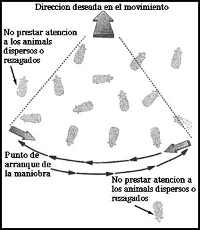
\includegraphics{figura111_sm}\\
\end{figure}

\begin{figure}
Figura 1.1.2\\
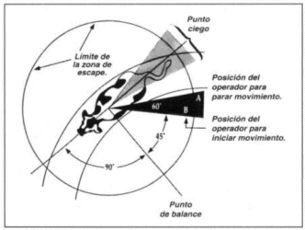
\includegraphics{figura112_sm}\\
\end{figure}

\begin{figure}
Figura 1.1.3\\
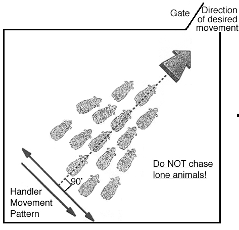
\includegraphics{figura113_sm}\\
\end{figure}

\begin{figure}
Figura 1.1.4\\
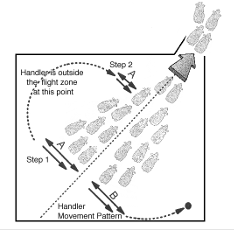
\includegraphics{figura114_sm}\\
\end{figure}


\pagebreak

\subsection{Sección 2}
\label{subsubsection:seccion2}

\begin{figure}
\begin{verbatim}
Figura 2.1.1

$K\_app\_dependencies = [
    {   module: "Boids", 
        description: "Boids Demo App.",
        path: "",
        files: [
            { name: "brain/behavior\_modifier.js",  
               description: "Self protection behaviors." },
            { name: "brain/behavior.js",           
               description: "Abstract Behavior." },
            { name: "brain/security\_behavior.js",  
               description: "Self protection behaviors." },
            { name: "brain/itinerant\_behavior.js", 
               description: "Definition of itinerant behaviors." },
            { name: "brain/behavior\_group.js",     
                description: "Group of related behaviors." },
            { name: "brain/brain.js",              
               description: "Boid Brain." },
            { name: "boid.js",                     
               description: "One Boid." },
            { name: "world\_interface.js",          
               description: "World Interface." },
            { name: "boid\_editor.js",              
               description: "Boid panel editor." },
            { name: "world.js",                    
               description: "The world where all boids live." },
            { name: "main.js",                     
               description: "main function." },
        ]
    }
]
\end{verbatim}
\end{figure}


\subsection{Sección 3}
\label{subsubsection:seccion3}

Figura 3.1.1\\
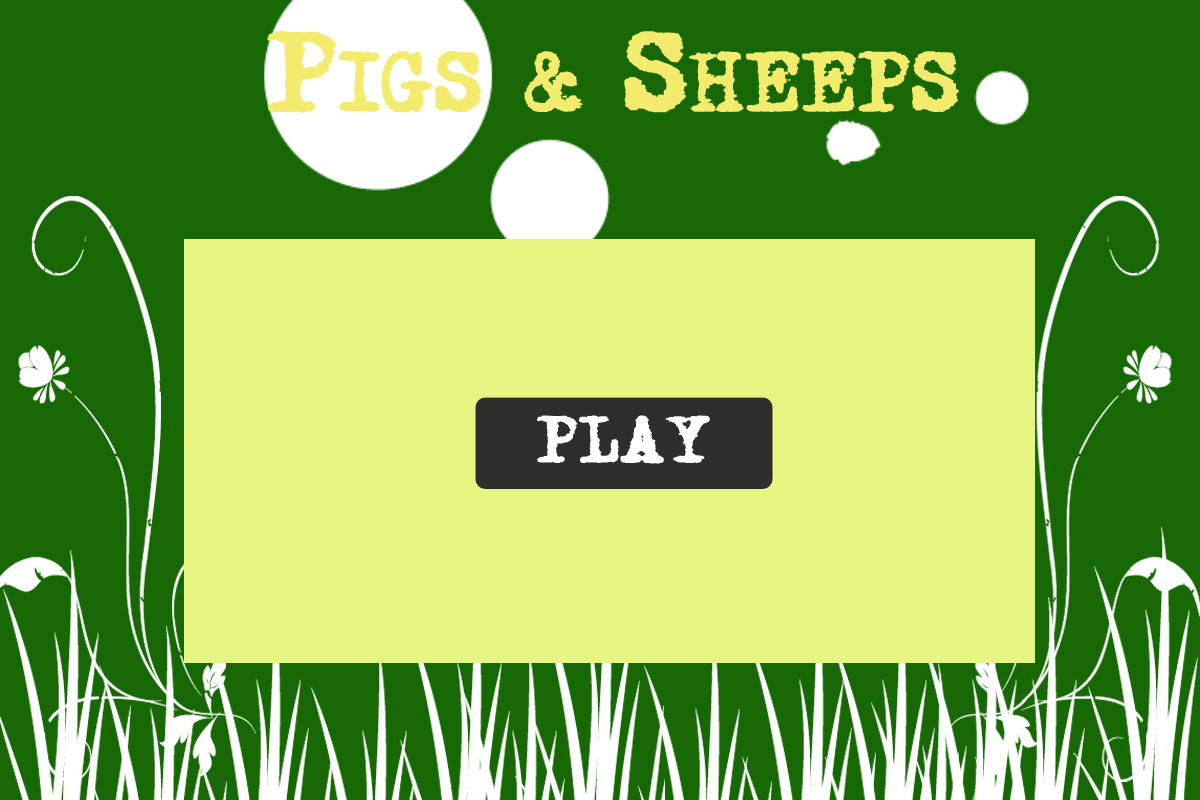
\includegraphics[scale=0.32]{figura311}\\

Figura 3.1.2\\
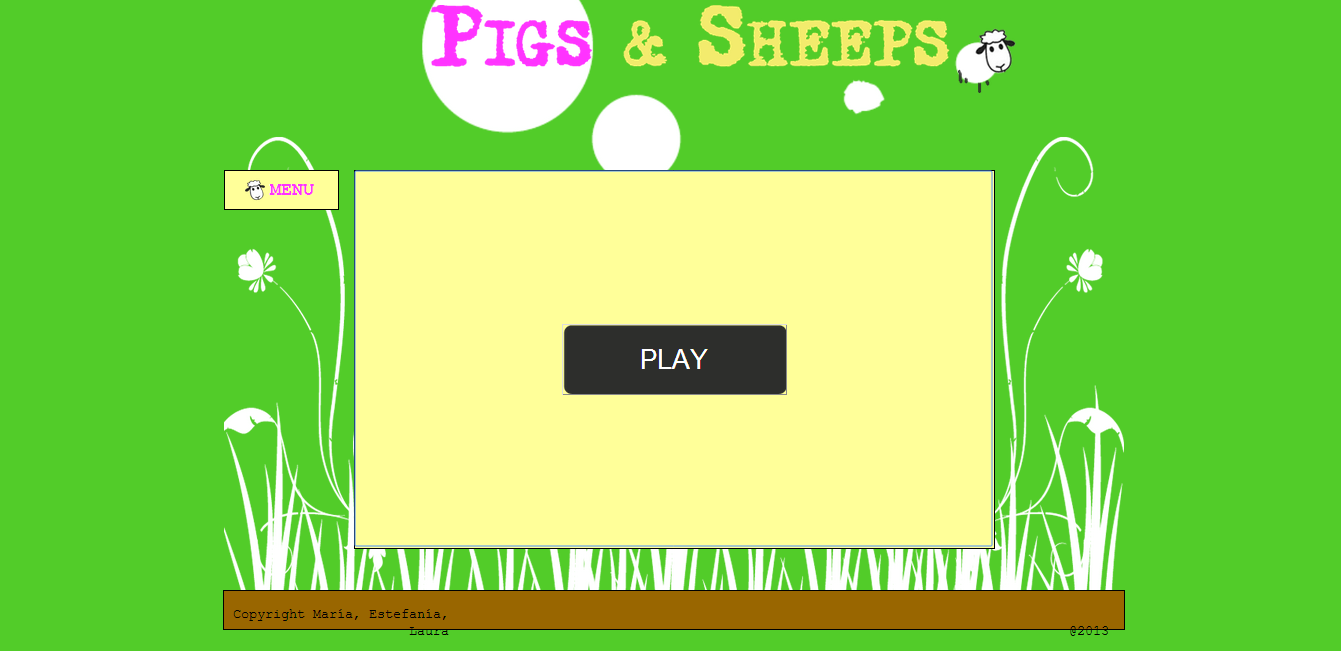
\includegraphics[scale=0.33]{figura312}\\

Figura 3.1.3\\
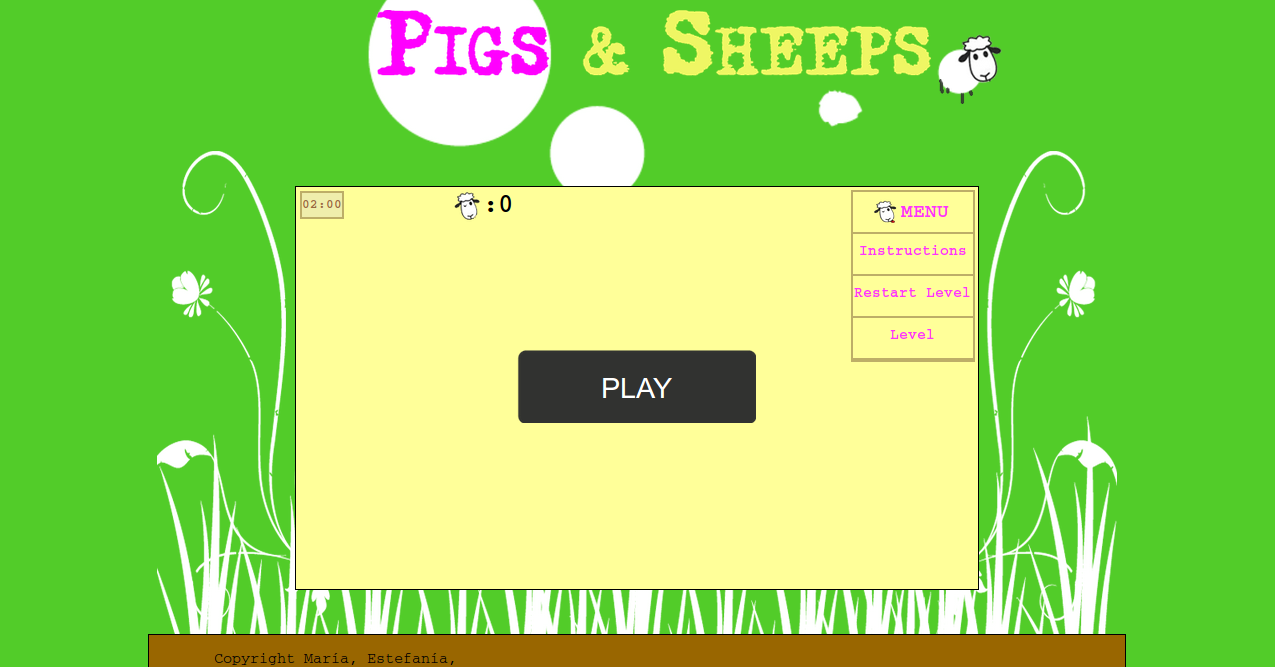
\includegraphics[scale=0.33]{figura313}\\


Figura 3.2.1\\
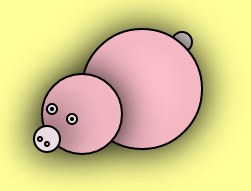
\includegraphics{figura321}\\

Figura 3.2.2\\

\includegraphics{figura322}\\

Figura 3.2.3\\

\includegraphics{figura323}\\

Figura 3.2.4\\
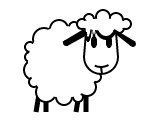
\includegraphics{figura324}\\

Figura 3.2.5\\
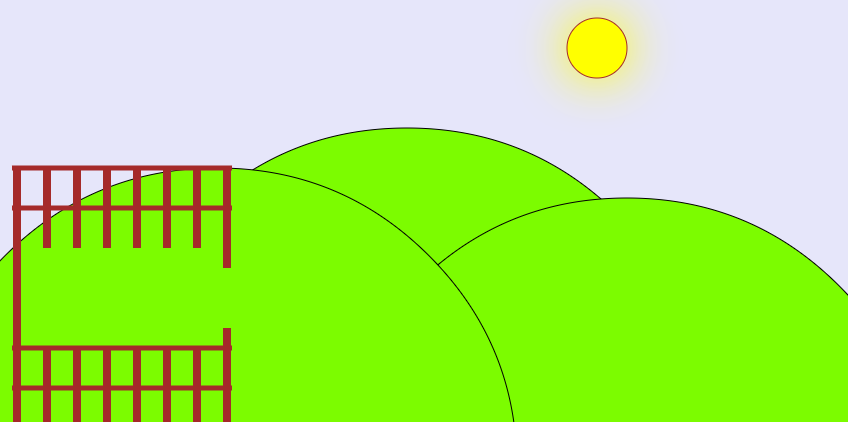
\includegraphics[scale=0.33]{figura325}

\pagebreak
\subsection{Sección 4}
\label{subsubsection:seccion4}

\begin{figure}
Figura 4.1.1
\begin{verbatim}
 function Vehicle(mass, number\_of\_wheels){
  this.mass = mass // In kg 
  this.number\_of\_wheels = number\_of\_wheels
  Vehicle.prototype.yield(this)
}

boeing = new Vehicle(20000, 8, function(newly\_created\_airplane){
  newly\_created\_airplane.wings = 2  // This is a singleton attribute
})
\end{verbatim}
\end{figure}


\begin{figure}
Figura 4.1.2
\begin{verbatim}
 var animal = function(limbs, name){
  if (limbs<5)
      return function Mammal(main\_food){
          this.name  = name
          this.limbs = limbs
          this.main\_food = main\_food
      }
    else
      return function Spider(number\_of\_teeth){
          this.name  = name
          this.limbs = limbs
          this.number\_of\_teeth = number\_of\_teeth
      }
}

dog = new (Animal("Tim", 4))("meat")
\end{verbatim}
\end{figure}


Figura 4.1.3\\
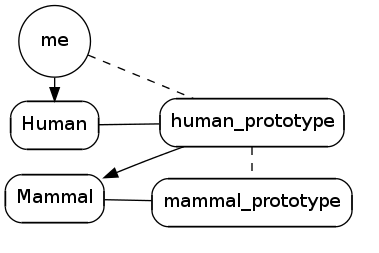
\includegraphics[scale=0.33]{figura413}\\


\begin{figure}
Figura 4.2.1.1 
\begin{verbatim}
 var default\_config = {
           geo\_data: {
               position: new Vector(Math.floor(Math.random()*400), 
                                    Math.floor(Math.random()*400)),
               velocity: new Vector(Math.floor(Math.random()*40),
                                    Math.floor(Math.random()*40)),
               acceleration: new Vector(0,0)
           },
           colour: "blue",

           brain: new Brain(that),
           vel\_max: 50,
           mass: 2,
           vision: {radius: 100, angle: 130 * Math.PI / 180},

           force\_limits: {
               thrust: 20,
               steering: 50,
               braking: 70
           }
}
\end{verbatim}
\end{figure}


figura 4.2.1.2\\
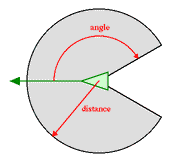
\includegraphics{figura4212}\\


\begin{figure}
Figura 4.2.3.1
\begin{verbatim}
 Sheep.prototype.sheep\_limits = function() {
    var x\_axis = this.geo\_data.position.Coord[0]
    var y\_axis = this.geo\_data.position.Coord[1]

    if(y\_axis >= 800 && x\_axis >= 170 || 
       y\_axis >= 800 && x\_axis <= 274){
           if(this.first\_time == 0){
                 this.my\_world.max\_score = true
                 return
           }
           else
                 return
    }
    if(x\_axis <= -445 || x\_axis >= 395)
           this.geo\_data.velocity.Coord[0] = 0
    if (y\_axis >= 800 || y\_axis <= 0) {
            this.geo\_data.velocity.Coord[1] = 0
    }
}
\end{verbatim}
\end{figure}


\begin{figure}
Figura 4.2.3.3
\begin{verbatim}
 Sheep.prototype.first\_draw = function() {
    var canvas = document.createElement('canvas');
    canvas.width = 24;
    canvas.height = 24;

    var ctx = canvas.getContext('2d');
}
\end{verbatim}
\end{figure}


\begin{figure}
Figura 4.2.3.4
\begin{verbatim}
 Sheep.prototype.draw = function(ctx){
    var p = this.geo\_data.position
    var v = this.geo\_data.velocity
    var a = this.geo\_data.acceleration
    var radius = 10
    var scale = 1 - p.get\_coord(1) / 3000
    var x = this.geo\_data.velocity.get\_coord(0)

    ctx.save()
    ctx.scale( scale, scale / 2 )

    if(x < 0) {
       ctx.drawImage(this.image, 
                     p.get\_coord(0),
                     p.get\_coord(1))
    }
    else
       ctx.drawImage(this.image\_left, 
                     p.get\_coord(0),
                     p.get\_coord(1))

    ctx.restore()
}
\end{verbatim}
\end{figure}


\begin{figure}
Figura 4.2.4.1
\begin{verbatim}
 MouseCoordinates.prototype.do_onclick = function (ev, el) {
   this.X = ev.pageX - screener.offsetLeft
   this.Y = ev.pageY - screener.offsetTop
   this.device.move\_shepherd(this.X, this.Y)
}
\end{verbatim}
\end{figure}


 
figura 4.3.3.1\\
- gráfico de velocidades y aceleraciones -\\


\begin{table}
\caption{Comportamientos. Cuadro 4.3.2.1}
% title of Table
%\centering
% used for centering table
\begin{tabular}{| p{4cm} | p{7cm} | p{4cm} |} % centered columns (4 columns)

\hline\hline %inserts double horizontal lines
Nombre de la técnica & Boid cerdito & Boid oveja \\ [0.5ex] % inserts table
%heading
\hline % inserts single horizontal line
% inserting body of the table
Técnica del limpiaparabrisas & El pastor debe moverse en zig-zag detrás de la manada, para mantenerlos en línea recta. & Las ovejas deben de agruparse y moverse en línea recta.\\
Zona de fuga & El cerdito se encuentra en la zona de fuga de la oveja. & La oveja se agita y se enfrenta a él. \\
Moverlos en una manga & El cerdo debe de situarse enfrente del punto de equilibrio & Las ovejas avanzan hacia atrás. \\
Sacar a las ovejas del corral con un controlador & El cerdo se sitúa  a 90º detrás del ganado. Los movimientos deben de ser perpendiculares a los del ganado, hacia delante y hacia atrás sobre la barra transversal de una gigante T. & las ovejas salen en 
manada del corral. \\ [1ex] % [1ex] adds vertical space
\hline %inserts single line
\end{tabular}
\label{table:nonlin} % is used to refer this table in the text
\end{table}

\begin{figure}
Figura 4.3.2.2
\begin{verbatim}
SheepBehavior.prototype.desired\_velocity = function(){
 var arrival\_distance
 try{
    arrival\_distance = this.target_at().module()
 }catch(err){
    arrival\_distance = 0
 }
 var scale = 1
 if(arrival\_distance >= 100){
    scale = 0
 }
 else{
    scale = arrival\_distance / 100
 }

 return (new Vector(this.target\_at().unit().scale(- scale 
                     * this.me.vel_max)))
}
\end{verbatim}
\end{figure}


\begin{figure}
Figura 4.4.1
\begin{verbatim}
World.prototype.move_shepherd = function (screen_x, screen_y) {
   if (!this.shepherd)
       return
   var behaviour = this.shepherd.brain.get_behavior("seek mouse", null)
   var x = screen_x - 425
   var y = 500 - screen_y
   var scale = 1 - y / 3000

   behaviour.set_target_at( x / scale, 2 * y / scale)
}
\end{verbatim}
\end{figure}


\begin{figure}
Figura 4.4.2
\begin{verbatim}
World.prototype.check_level = function() {
    if(this.level == 1 && this.points == 5){
           this.is_finished = true
           this.currentState.requested = this.state.suspended
           this.clock.pause()
           this.winner_pig()
    }
}
\end{verbatim}
\end{figure}


\begin{figure}
Figura 4.4.3
\begin{verbatim}
World.prototype.running_steady = function(processors_time){
       this.now = processors_time || new Date()
       this.coord_x = this.mouse_coordinates.get_mouse_X()
       this.coord_y = this.mouse_coordinates.get_mouse_Y()

    score_number.style.float = "right"
    score_number.style.fontSize = "24pt"
    score_number.style.marginTop = "5px"
    score_number.style.fontWeight = "bold"
    score_number.innerHTML = ":" + this.points

    this.check_level()
    if(this.is_finished == false)
       this.draw()
}
\end{verbatim}
\end{figure}


\begin{figure}
Figura 4.5.1
\begin{verbatim}
Galactus.prototype.start_world = function() {
   this.world = new World(this.view)
   this.world.level = 1

   this.handler.addPort("restart_game", this)
   
   this.countdown()
   this.playSound()

   var pig = this.world.new_boid_of(Pig, function(config) {
       config.brain.activate("seek mouse", null)
   })

   this.world.shepherd = pig

   var sheeper = [ ]
   for (var i=0; i<30; i++) {
        sheeper.push( this.world.new_boid_of(Sheep, 
           function(config){
             config.geo_data.position = new Vector(
                 Math.floor(Math.random()*400), 
                 Math.floor(Math.random()*400) )
             config.geo_data.velocity = new Vector(
                 Math.floor(Math.random()*20), 
                 Math.floor(Math.random()*20)  )
             config.geo_data.acceleration = new Vector(0,0)
             config.vel_max = 70
             config.vision = {radius: 100, angle: 80 * Math.PI / 80}           
             config.force_limits = {
                   thrust: 50,
                   steering: 50,
                   braking: 100
             }
             config.brain.activate("alignment")
             config.brain.activate("sheep", pig)
      }))
  }
   this.world.start()
}
\end{verbatim}
\end{figure}



\subsection{Sección 5}
\label{subsubsection:seccion5}

\begin{figure}
Figura 5.1.1\\
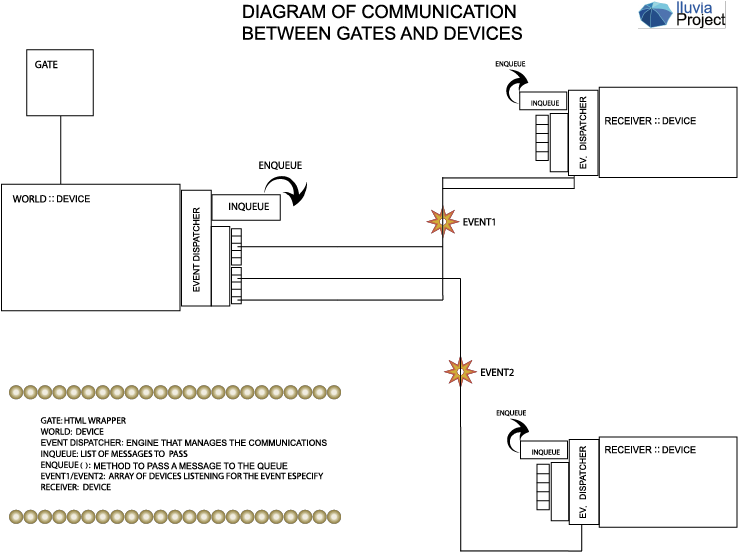
\includegraphics[scale=0.33]{figura511}\\
\end{figure}


\begin{figure}
Figura 5.1.2
\begin{verbatim}
     Button.prototype = new Gate
     Button.prototype.constructor = Button

     function Button(element){

        try {
            if (arguments.length)
                Gate.call(this, element)// LLama al superconstructor de Gate.
        } catch (e) {
            if (\$K_debug_level >= \$KC_dl.DEVELOPER)
                alert("No event handlers were found.\nException: " 
                       + e.toSource())
        }
     }

     Button.prototype.do_onclick   = function(event, element){
        alert("You have made click.")
     }

     var b = new Button(id_of_html_element, null, {
         do_onmouseover: function(event, element) {
             alert("Hello")
         }
     })
\end{verbatim}
\end{figure}
 
\begin{figure}
figura 5.2.1
\begin{verbatim}
[function(){
    this.gate.panel.style.height = "" + 250 +"px" 
}; ],
\end{verbatim}
\end{figure}


\begin{figure}
figura 5.2.2
\begin{verbatim}
[function (){
    if( this.menu_height >= 50 && this.menu_height<=205)
       this.menu_height+=5
    this.gate.panel.style.height = "" + this.menu_height +"px"
};],
\end{verbatim}
\end{figure}


\begin{figure}
figura 5.2.3
\begin{verbatim}
[function(){
    if( this.menu_height >=55 ){         
        this.menu_height-=5
    this.gate.panel.style.height = "" + this.menu_height +"px"
},],
\end{verbatim}
\end{figure}

